%!TEX root = ../thesis.tex
%*******************************************************************************
%****************************** Second Chapter *********************************
%*******************************************************************************

\chapter{Towards Non-Orthogonal Multiple Access for Next-Gen Wireless Networks} \label{Chapter:noma}

\ifpdf
    \graphicspath{{Chapter2/Figs/Raster/}{Chapter2/Figs/PDF/}{Chapter2/Figs/}}
\else
    \graphicspath{{Chapter2/Figs/Vector/}{Chapter2/Figs/}}
\fi

Non-Orthogonal Multiple Access (NOMA) represents a shift in multiple access technologies, enhancing spectrum efficiency and user capacity over traditional methods. This chapter explores Power-Domain NOMA, addressing its technology, performance, and challenges in uplink multi-user detection. It critiques the limitations of Successive Interference Cancellation (SIC) and proposes Maximum Likelihood detection as a superior alternative.

\section{Enabling Massive Connectivity for Next-Gen Wireless Networks}\label{section}


The current landscape of wireless communications is dominated by fourth-generation (4G) and fifth-generation (5G) networks. 4G has been the backbone of modern mobile internet, providing substantial improvements in speed and connectivity over its predecessors. However, as technology progresses, 5G has begun to take the spotlight, offering even faster speeds, reduced latency, and greater capacity. 5G networks support a variety of new applications, including enhanced mobile broadband, massive machine-type communications (mMTC), and ultra-reliable low-latency communications (URLLC).

Despite these advancements, the rapid increase in the number of mobile users and Internet-enabled devices poses a significant challenge. By the end of 2024, Cisco predicts that the number of mobile users will reach 13.1 billion, and the number of Internet-enabled devices will soar from 18.4 billion in 2018 to 29.3 billion \cite{cisco2020report}. This explosive growth will gradually overwhelm the connectivity capabilities of both 4G and 5G networks. Additionally, this increasing trend shows no sign of slowing down in the next decade since this demand is caused only by around 70\% of the global population \cite{cisco2020report}. Therefore, providing massive access is one of the most important targets for next generation wireless networks, namely the sixth-generation (6G). Currently, the research on 6G is being carried out on the global stage, e.g., the ``6G Flagship'' in Finland \cite{oulu2021sixg}, ``6G Hubs'' in Germany, ``Broadband Communications and New Networks'' in China, Terahertz (THz) communication studies in the USA, to name a few. To support future Internet of Everything (IoE) and Mobile Internet, 6G has several critical performance targets \cite{zhang2019wireless}: a) The peak data rate needs to be at least one terabit per second; b) the air interface latency shall range from 0.01 to 0.1 millisecond for users with high mobility; c) the connectivity density shall be 10 times larger than in current 5G systems; d) the spectral efficiency (SE) and energy efficiency (EE) have to be 5-10 and 10-100 times higher than for 5G, respectively; and e) the reliability has to be higher than 99.99999\%.

In order to achieve these stringent targets, one of the most fundamental advancements needed is the design of sophisticated multiple access techniques, referred to as Next Generation Multiple Access (NGMA). The transition from Orthogonal Multiple Access (OMA) to Non-Orthogonal Multiple Access (NOMA) is already expected to occur in the eMBB use cases of 5G to increase system throughput. This evolution will be even more crucial for 6G to handle the vast number of devices and the high data rate requirements. NGMA will play a pivotal role in enabling the scalability, efficiency, and performance required for the next wave of global connectivity demands. The following section will explore into the currently employed multiple access techniques alongside the emerging NGMA \cite{nagma2}.

\section{The Evolution of Multiple Access Techniques in Wireless Networks}

Wireless communication fundamentally relies on the efficient use of radio resources—time and frequency—to transmit data from one device to another. The fundamental physical radio resources are time and frequency, which are usually interpreted as physical degrees of freedom to transmit data. The problem of multiple access arises when multiple users need to be served with limited (or scarce) degrees of freedom in the radio resource. It is intuitive to consider dividing the available degrees of freedom in an orthogonal way so that each user’s transmission will not interfere with another.

Looking back at the development history of wireless communications, multiple access techniques have been key enablers. Depending on whether each user is allocated orthogonal resources or not, the current multiple access techniques can be loosely classified into two categories, namely orthogonal transmission strategies and non-orthogonal transmission strategies. In particular, given their advantages of low complexity and interference-avoidance, orthogonal transmission strategies have been extensively employed in practical wireless communication systems. These include Frequency Division Multiple Access (FDMA) in the first generation (1G), where the available spectrum is partitioned into non-overlapped frequency sub-bands, each accommodating one digital data stream. Time Division Multiple Access (TDMA) in the second generation (2G) partitions time into slots, each serving a digital data stream in a round-robin fashion \cite{noma1}. Code Division Multiple Access (CDMA) with orthogonal codes in the third generation (3G) and Orthogonal Frequency Division Multiple Access (OFDMA) in 4G allocate orthogonal frequency/time/code resource blocks \cite{noma2}. OFDMA is a multi-carrier multiple access scheme based on the Orthogonal Frequency Division Multiplexing (OFDM) waveform, which enables tight and orthogonal frequency-domain packing of the subcarriers with a subcarrier spacing inverse to the symbol duration. With OFDMA, the time and frequency plane is divided into a two-dimensional raster, each transmitting a modulated symbol that belongs to one data stream.

The introduction of code and spatial domains has further expanded the degrees of freedom in resource allocation. Similarly, Spatial Division Multiple Access (SDMA) uses the spatial domain to separate users based on their physical location, which can be managed either orthogonally or non-orthogonally through various precoding techniques \cite{kizilirmak2016noma}.

Despite the clear benefits of OMA schemes, such as simplified transceiver design and reduced co-channel interference, they have notable limitations. Primarily, the number of users that can be served simultaneously is capped by the available radio resources, and maintaining orthogonality requires complex user scheduling and feedback mechanisms, leading to increased signaling overhead \cite{liu2020noma}. However, given the ever-increasing number of wireless devices and the limited amount of available spectrum, conventional orthogonal transmission strategies have become inefficient due to their low spectral efficiency (SE) and the limited number of users/devices that can be supported due to inflexible resource allocation. As a result, to handle the challenging emerging heterogeneous services and applications (e.g., virtual reality (VR), augmented reality (AR), and Industry 4.0), non-orthogonal transmission strategies are widely considered to be a promising solution and have drawn significant research interests in recent years \cite{NAGMA}.

The goal of NAGMA is to enable a tremendous number of users/devices to be efficiently and flexibly connected with the network over the given wireless radio resources. Different from orthogonal transmission strategies, the key idea of non-orthogonal transmission strategies is to allow different users to share the same resource blocks. To deal with the resulting interference caused by the non-orthogonal resource allocation, additional techniques have to be employed at the transmitters and receivers, including but not limited to superposition coding (SC), rate splitting (RS), successive interference cancellation (SIC), and message passing (MP). Although the non-orthogonal transmission strategies increase the transmitter and receiver complexity, significant benefits can be achieved, such as supporting massive connectivity, achieving high SE and EE, and guaranteeing user fairness. As a result, compared with orthogonal transmission strategies, the aforementioned benefits make non-orthogonal transmission strategies promising candidates for NGMA \cite{nagma2}.
\subsection{Considerations for Next Generation Multiple Access Design}

In this subsection, we identify several new considerations that need to be taken into account for \textit{NGMA design}, addressing the specific needs and challenges that emerge with the evolution of cellular networks and IoT integration.

\begin{enumerate}
    \item \textbf{Massive Access}: With the increasing demand for expanding cellular connectivity, as well as the burgeoning Internet of Things (IoT) market, next-generation cellular networks will be characterized by an exceptionally large number of users—a scenario also referred to as \textit{massive connectivity} or \textit{massive access}. Traditional information-theoretic results on multiple access schemes mostly focus on finding capacity limits for an infinite coding blocklength and a fixed number of users. However, for massive access channels, where the number of users grows with the blocklength, these fundamental limits need to be revisited. The authors of a key study proposed the notion of a \textit{many-access channel} (MnAC), modeling a channel with a single receiver and multiple transmitters, the number of which grows unboundedly with the blocklength \cite{NAGMA}. New notions of achievable message length and symmetric capacity were introduced, where separate identification and decoding were shown to be capacity-achieving.
    
    \item \textbf{Short-Packet Transmission}: Another critical feature to consider for NGMA is \textit{short-packet transmission}, particularly relevant in IoT applications where the coding blocklength is finite and short due to the low latency requirements. Research in this area has derived the maximum channel coding rate for a given blocklength and error probability, highlighting the rate gap compared to scenarios with infinite coding blocklength \cite{nagma2}. Extending these results to a regime with a large yet finite number of users and a finite coding blocklength remains an open problem. This gap indicates a significant area for future research, as approaching these fundamental limits with practical transmission and multiple access schemes will be crucial for the successful deployment of NGMA technologies in real-world scenarios.
\end{enumerate}

Both of these considerations—\textit{massive access} and \textit{short-packet transmission}—point towards a future where NGMA must be adaptable, robust, and capable of handling increasingly complex communication environments.
\subsection{Possible Candidates for Next Generation Multiple Access}

As discussed in the previous subsections, the trend of \textit{NGMA} is to transition from orthogonality to non-orthogonality, serving multiple users/devices by allowing them to share the same resources instead of allocating them dedicated orthogonal resources. This Rapidly growing user base can only be supported to a limited extent by traditional orthogonal resources, calling for the development of non-orthogonal transmission schemes for NGMA. Below, we introduce some potential candidates for NGMA based on the concept of non-orthogonality, along with their technical foundations:

\begin{enumerate}
    \item \textit{Power-Domain NOMA (PD-NOMA)}: The key idea of PD-NOMA is to serve multiple users within the same time/frequency/code resources and distinguish them in the power domain. Superposition coding (SC) and successive interference cancellation (SIC) are two key technologies in PD-NOMA, which have been proven to be capacity-achieving in the single-antenna broadcast channel (BC) and multiple access channel (MAC) \cite{noma1}. PD-NOMA can be straightforwardly integrated with OFDM, as demonstrated by the multiuser superposition transmission (MUST) technique, which has been incorporated into LTE-A for supporting two users on the same OFDMA subcarrier. Another application of PD-NOMA is layered division multiplexing (LDM), included in the digital TV standard (ATSC 3.0) for delivering multiple superpositioned data streams for TV broadcasting \cite{noma3}.
    
    \item \textit{Code-Domain NOMA (CD-NOMA)}: Inspired by CDMA, CD-NOMA serves multiple users via the same time/frequency resources but employs user-specific spreading sequences which may be sparse or have low cross-correlation. At the receiver, multiuser detection (MUD) is usually carried out in an iterative manner using message passing (MP) based algorithms. The family of CD-NOMA schemes includes Low-Density Signature (LDS)-CDMA, LDS-OFDM, Sparse Code Multiple Access (SCMA), and Pattern Division Multiple Access (PDMA) \cite{liu2020noma}.
    
    \item \textit{Space Division Multiple Access (SDMA)}: With the advancement of multi-antenna techniques, MIMO communication has become a cornerstone in current 5G standards and future wireless networks. By utilizing multiple antennas at transmitters and/or receivers, additional spatial degrees of freedom (DoFs) can be exploited, distinguishing multiple users/devices in the same time/frequency/code domain in the spatial domain. The most commonly employed method for SDMA is linear precoding (LP), which effectively mitigates inter-user interference by exploiting spatial DoFs to design suitable transmit and/or receive beamformers \cite{noma2}.
    
    \item \textit{Rate Splitting Multiple Access (RSMA)}: RSMA is a newer non-orthogonal multi-antenna transmission scheme that relies on the rate splitting technique. The transmitter splits each user's message into a common message intended for all served users and private messages. The constructed common message and the remaining private messages are transmitted via beamformers, similar to SDMA. At the receivers, the common message is decoded first with private messages treated as interference, followed by the subtraction of the common message from the received signal (using SIC), and then decoding the intended private message. RSMA provides more flexibility in mitigating interference compared to SDMA, offering significant advantages in overloaded network scenarios \cite{NAGMA}.
\end{enumerate}

Given these potential candidates, this project focuses on exploring PD-NOMA to develop NGMA, as NOMA offers a higher degree of compatibility and flexibility. This enables the seamless integration of NOMA with other components of next-generation networks, such as multi-antenna techniques, challenging application scenarios, and other physical layer techniques, details of which will be elaborated in the following section.
\section{Power Domain Non-Orthogonal Multiple Access (PD-NOMA)}

In the evolving landscape of wireless communications, efficiently managing the scarce spectral resources to accommodate the exponential growth in the number of devices and data traffic is paramount. PD-NOMA emerges as a transformative solution in this context, fundamentally changing how spectrum resources are utilized by allowing multiple users to share the same spectral resources distinguished by different power levels. This technique diverges from traditional orthogonal access methods, where resources such as time, frequency, and code are allocated exclusively to individual users, often leading to under-utilization of these precious assets. By assigning different power levels to user signals that overlap in both time and frequency, PD-NOMA can significantly increase the spectral efficiency of a network. Additionally, it also improves user fairness by ensuring that users with poor channel conditions are not left behind. This capability is especially critical in high-demand environments such as urban centers and for emerging technologies that require massive connectivity, such as the IoT.


In the following sections, we will explore the key components and operational aspects of PD-NOMA, including superposition coding, successive interference cancellation, and its application in uplink and downlink scenarios.
\subsection{Superposition Coding (SC)}

Superposition Coding (SC) is a fundamental technique in PD-NOMA, which enables a single transmitter to simultaneously communicate information to several receivers by varying the power levels assigned to each user's signal. This method is essential in broadcasting scenarios where multiple users receive the same channel's information, such as in digital television or certain types of data streaming.

To implement SC, the transmitter employs two point-to-point encoders that map the input bits of each user to output bit sequences. These sequences are then transmitted over the same channel but are modulated at different power levels. The encoding functions for the users are defined as:
\begin{itemize}
    \item User 1: \( f_1:\{0,1\}^{R_1} \rightarrow \mathcal{C}^T \)
    \item User 2: \( f_2:\{0,1\}^{R_2} \rightarrow \mathcal{C}^T \)
\end{itemize}
\begin{figure}[H]
    \centering
    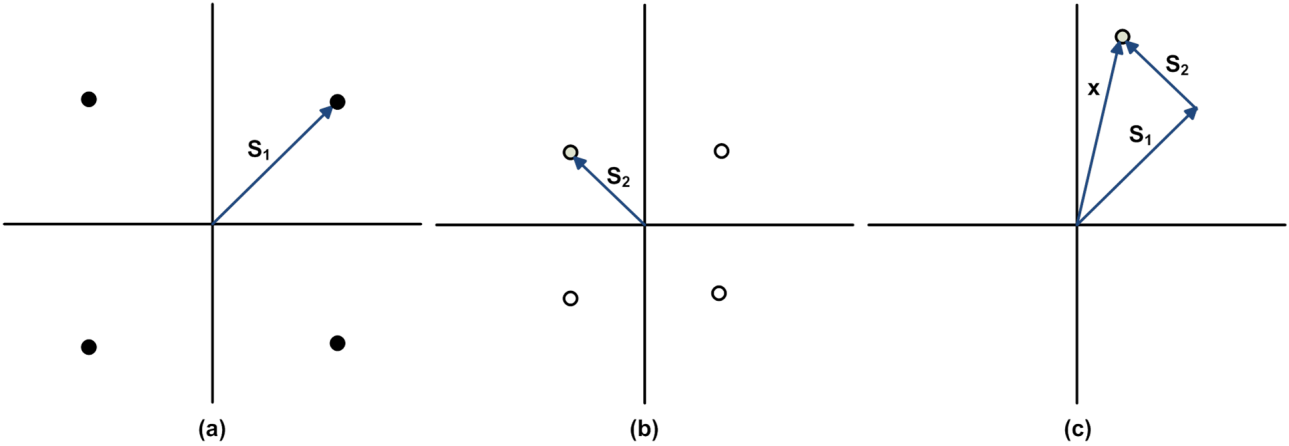
\includegraphics[width=1\linewidth]{SC.png}
    \caption{An example of SC encoding (a) signal constellation of user 1 (b) signal constellation of user 2 (c)
constellation of superposed signal.}
    \label{fig:enter-label}
\end{figure}
where \( R_1 \) and \( R_2 \) denote the transmission rates for User 1 and User 2, respectively, \( T \) represents the block length, and \( \mathcal{C} \) is the coding library used \cite{noma3}. The encoded sequences \( S_1(n) \) and \( S_2(n) \) are combined using the superposition principle:
\[
X(n) = \sqrt{P\alpha_1}S_1(n) + \sqrt{P\alpha_2}S_2(n)
\tag{2.1}\]
Here, \( \alpha_1 \) and \( \alpha_2 \) are the power fractions allocated to User 1 and User 2, respectively, with the constraint \( \alpha_1 + \alpha_2 = 1 \).

Superposition coding is noted for its capacity-achieving properties on scalar Gaussian broadcast channels and its ability to maximize network throughput by efficiently using the available bandwidth and power. It adjusts power levels according to the varying channel conditions of different users, optimizing the overall communication efficiency. SC has been integrated into various practical applications, including LTE-A through Multiuser Superposition Transmission (MUST), supporting multiple users on the same OFDMA subcarrier, and in digital TV standards like ATSC 3.0, enabling the delivery of multiple data streams simultaneously \cite{ding2017survey}.

\subsection{Successive Interference Cancellation (SIC)}

\textit{Successive Interference Cancellation} (SIC) is a decoding technique critical in environments where signals from multiple users are superposed, such as in PD-NOMA. SIC exploits the differences in signal strengths to sequentially decode overlapping signals transmitted over the same channel. The process involves initially ordering the signals by strength, decoding the strongest signal first while treating the others as noise, and then subtracting the decoded signal from the combined signal to facilitate the decoding of the next strongest signal, this process is done iteratively until all users are decoded \cite{kizilirmak2016noma}. this is outlined in \autoref{fig:sic1}. 
\begin{figure}[H]
    \centering
    \includegraphics[width=0.5\linewidth]{sic1.png}
    \caption{SIC receiver.}
    \label{fig:sic1}
\end{figure}
The effectiveness of SIC in enhancing decoding accuracy and spectral efficiency makes it essential for managing interference among signals in dense user environments. The procedural implementation for a two-user scenario involves the following mathematical steps:

\begin{enumerate}
    \item At user 1, the decoder \( g_1: \mathcal{C}^T \rightarrow \{0,1\}^{R_1} \) decodes the message \( S_1(n) \) while considering \( S_2(n) \) as noise.
    \item User 2's decoder successively recovers its message by:
    \begin{itemize}
        \item Decoding user 1's message \( S_1(n) \) using \( g_1 \).
        \item Subtracting the decoded signal, adjusted for the channel gain and power \( \sqrt{P\alpha_1 h_2}S_1(n) \), from the received signal \( Y_2(n) \) to get:
        \[
        Y'_2(n) = Y_2(n) - \sqrt{P\alpha_1 h_2}S_1(n),
\tag{2.2}        \]
        where \( h_2 \) represents the complex channel gain at user 2.
        \item Decoding user 2's message \( S_2(n) \) using another decoder \( g_2: \mathcal{C}^T \rightarrow \{0,1\}^{R_2} \) applied to \( Y'_2(n) \).
    \end{itemize}
\end{enumerate}
\autoref{fig:SIC} presents the technique for decoding the superposed signal at the receiving side. Here, the constellation point of user 1 is decoded
first from the received signal. Then, the decoding of the constellation point of user 2 is performed
with respect to decoded constellation point of user 1.
\\The success of SIC depends on the perfect cancellation of the signals in the iteration steps. The transmitter should accurately split the power between the user information waveforms and superimpose them. The methodology for power split differs for uplink and downlink channels.
\begin{figure}[H]
    \centering
    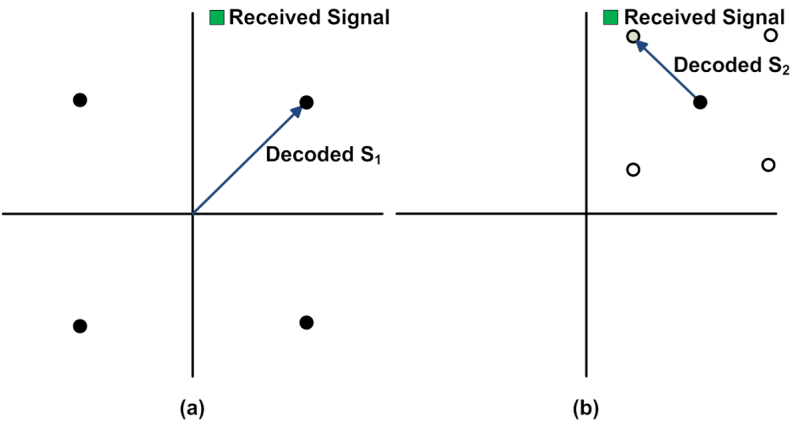
\includegraphics[width=0.7\linewidth]{Chapter2/Figs/1609.png}
    \caption[An example of SC decoding.]{An example of SC decoding (a) decoding the signal of user 2 (b) decoding the signal of user 1.}
    \label{fig:SIC}
\end{figure}
 
\subsection{Downlink NOMA Transmission}
We consider a simple NOMA system consisting of a single base station (BS) and two users, each equipped with a single antenna. Suppose that $x_1$ and $x_2$ are the signals to be transmitted from the BS to users 1 and 2, respectively. The BS transmits the superposition coded signal as:
\[
s = \sqrt{P_1} x_1 + \sqrt{P_2} x_2, 
\tag{2.3}\]
where $P_i$, for $i = 1, 2$, is the transmit power for user $i$, and the message signal $x_i$, for $i = 1, 2$, is of unit power, i.e., $E\{|x_i|^2\} = 1$, with $E\{\cdot\}$ as the expectation operator. The total transmit power for users 1 and 2 can then be written as $P = P_1 + P_2$. In practice, for a particular system setting, $P$ is predefined and is thus divided into $P_1$ and $P_2$ according to the adopted power allocation (PA) scheme. The received signal at user $i$ can be represented as:
\[
y_i = h_i s + n_i, \tag{2.4}
\]
where $h_i$ is the channel gain between the BS and user $i$, and $n_i$ represents the Gaussian noise plus interferences with power spectral density $N_{f,i}$. For a multi-cell scenario, the inter-cell interference is also included in $n_i$.
Successive Interference Cancellation (SIC) is employed at the receivers to separate the signals of different users. The optimal decoding order for SIC is determined by the decreasing order of the strength of the users' channels, represented as $\frac{|h_i|^2}{N_{f,i}}$. This order allows each user to effectively eliminate interferences from signals of users whose decoding orders follow theirs. 

In this scheme, user 1, having the highest channel strength $\frac{|h_1|^2}{N_{f,1}}$, is referred to as the strong user, and user 2, with the least channel strength $\frac{|h_2|^2}{N_{f,2}}$, as the weak user. The base station (BS) periodically updates the SIC order based on channel state information (CSI) feedback from users. Users are informed of the latest SIC order by the BS. Generally, a user with weaker channel strength (weak user) receives a higher power allocation than a user with stronger channel strength (strong user) to enhance its signal-to-interference-plus-noise ratio (SINR).

In a typical 2-user NOMA scenario with $\frac{|h_1|^2}{N_{f,1}} > \frac{|h_2|^2}{N_{f,2}}$ (and hence $P_1 < P_2$), only user 1 performs SIC. It decodes the signal of user 2 ($x_2$) first and subtracts it from its received signal $y_1$ before decoding its own signal $x_1$. User 2 directly decodes its own signal $y_2$, treating $x_1$ as noise and thus not using SIC. 

If SIC is perfectly executed, the achievable data rate for the NOMA user $i$, $R_{i,\text{NOMA}}$, for a transmission bandwidth of 1 Hz can be written as:
\begin{align}
    R_{1,\text{NOMA}} &= \log_2 \left(1 + \frac{P_1 |h_1|^2}{N_{f,1}}\right), \tag{2.5a} \\
    R_{2,\text{NOMA}} &= \log_2 \left(1 + \frac{P_2 |h_2|^2}{P_1 |h_2|^2 + N_{f,2}}\right). \tag{2.5b}
\end{align}
%%The achievable sum capacity is given by:
%%\[
%%R_{\text{NOMA}} = R_{1,\text{NOMA}} + %%R_{2,\text{NOMA}}.
%%\]
Equations (2.5a) and (2.5b) suggest that the BS can adjust the data rate of each user by tuning the power allocation coefficients $\alpha_1 = \frac{P_1}{P}$ and $\alpha_2 = \frac{P_2}{P}$.

\textbf{Comparative Analysis with OMA:}
In the 2-user FDMA scenario, the transmission bandwidth of 1 Hz is divided such that user 1 uses $W_1$ Hz and user 2 uses the remaining ($1 - W_1$) Hz. The power allocation ratio remains the same as in the NOMA scheme. The achievable data rates for OMA users are expressed as:
\begin{align}
    R_{1,\text{OMA}} &= W_1 \log_2 \left(1 + \frac{P_1 |h_1|^2}{W_1 N_{f,1}}\right), \tag{2.6a} \\
    R_{2,\text{OMA}} &= (1 - W_1) \log_2 \left(1 + \frac{P_2 |h_2|^2}{(1 - W_1)N_{f,2}}\right). \tag{2.6b}
\end{align}
\autoref{fig:downlink} illustrates broadcast (BC) capacity/rate region comparison. The sum capacity for both OMA and NOMA can thus be written as:
\[
R_T = \sum_{k=1}^K R_k
\tag{2.7}\]
%%The achievable sum capacity for OMA is:
%%\[
%%R_{\text{OMA}} = R_{1,\text{OMA}} + %%R_{2,\text{OMA}}.
%%\]
This demonstrates that unlike NOMA, no OMA user suffers from the interference from the signal of the other user.
\begin{figure}
    \centering
    \includegraphics[width=1\linewidth]{downlink.png}
    \caption[Illustration of two-user downlink NOMA.]{Illustration of two-user downlink NOMA. (a) The signals of two users are multiplexed in the
power domain using the same time/frequency resource. (b) downlink NOMA transmission. (c) BC capacity/rate region comparison, 0 $\leq$ $p_1$ +$p_2$ $\leq$ 1W.}
    \label{fig:downlink}
\end{figure}
Note that we considered asymmetric channel condition (different channel gains for users 1 and 2) to perform the above comparisons on the data rate regions. We can find that OMA and NOMA provide identical data rate regions in a symmetric channel environment–– multiplexing in power domain does not become advantageous as the signals of both users undergo the same interference and noise [7]. Therefore, compared to OMA, NOMA in cellular downlink provides higher sum capacity and performs a better tradeoff between system efficiency and user fairness when the channel conditions are different among users. It is demonstrated that other forms of OMA techniques including TDMA and orthogonal frequency-division multiple access (OFDMA) are also significantly outperformed by NOMA in terms of throughput under different settings [8].
\\\textbf{Generalization to Multi-User Scenario:}
For a $K$-user downlink NOMA with $\frac{|h_1|^2}{N_{f,1}} > \frac{|h_2|^2}{N_{f,2}} > \cdots > \frac{|h_K|^2}{N_{f,K}}$ (and hence $P_1 < P_2 < \cdots < P_K$), the data rate for user 1 remains as in equation (3), while the data rate for any other user $k$ is:
\[
R_{k,\text{NOMA}} = \log_2 \left(1 + \frac{P_k |h_k|^2}{\sum_{j=1}^{k-1} P_j |h_k|^2 + N_{f,k}}\right). \tag{2.8}
\]

This model illustrates that while NOMA theoretically supports numerous users, practical implementations usually limit it to a few users in a cluster to maintain manageable bit error rates and computational demands, particularly for resource-constrained devices \cite{nomamath}.

\subsection{Uplink NOMA Transmission}
In uplink NOMA, multiple users transmit their signals to the base station (BS) within the same resource block. The BS employs Successive Interference Cancellation (SIC) to detect all the messages of the users. Notable differences between uplink NOMA and downlink NOMA include \cite{nomauplinkvsdownlink}:

\begin{itemize}
    \item \textbf{Transmit Power:} Unlike downlink NOMA, the transmit power of users in uplink NOMA may not differ significantly. It is primarily dictated by the channel conditions of each user. If the users' channel conditions vary greatly, their received Signal-to-Interference-plus-Noise Ratio (SINR) at the BS can be markedly different, regardless of their transmit power levels.
    \item \textbf{SIC Operations:} The mechanisms and interference experienced in uplink and downlink NOMA are distinct. In downlink NOMA, the SIC process involves canceling the interference from weaker users by first detecting the stronger user's signal, remodulating it, and subtracting it from the combined signal. Conversely, in uplink NOMA, the BS detects the stronger user's signal first by treating the other user as interference, then it remodulates and subtracts the detected signal to decode the weaker user's signal.
    \item \textbf{Performance Gain:} The performance advantage of NOMA over Orthogonal Multiple Access (OMA) varies between uplink and downlink scenarios. While downlink NOMA generally offers superior throughput performance, uplink NOMA provides improvements mainly in terms of fairness, particularly when channel conditions between users differ significantly.
\end{itemize}

Considering these aspects, the received signal at the BS is given by:
\[
y = \sum_{i=1}^2 \sqrt{P_i} h_i x_i + n, \tag{2.9}
\]
where $P_i$ is the transmit power for user $i$, with $E\{|x_i|^2\} = 1$, and $n$ represents the Gaussian noise plus interferences with power spectral density $N_f$. Typically, the BS broadcasts a downlink reference signal, based on which each user performs channel estimation and regulates their transmit power to either $P_1$ or $P_2$, depending upon their channel gains.

In this setting, user 1 is marked as the strong user experiencing a higher channel gain compared to user 2, the weak user. Upon receiving the superposed signal, the BS performs Successive Interference Cancellation (SIC) to separate the users' signals. The BS first decodes the signal of user 1 by treating the signal of user 2 as noise, then subtracts the decoded signal of user 1 ($\hat{x}_1$) from the received signal ($y$). From the remaining signal, the signal of user 2 ($\hat{x}_2$) is then decoded, \autoref{fig:uplink} illustrates this scenario.

Therefore, in uplink NOMA, user 1 experiences interference from user 2, whereas user 2 receives no interference from user 1 since user 1's signal is removed prior to decoding user 2's signal. This is in contrast to downlink NOMA, where user 2 experiences interference from user 1, while user 1 does not suffer interferences from user 1 since user 2's signal is removed prior to decoding user 1's signal.
\begin{figure}
    \centering
    \includegraphics[width=1\linewidth]{uplink.png}
    \caption[ Illustration of two-user uplink NOMA.]{ Illustration of two-user uplink NOMA. (a) The signals of two users are multiplexed in the
power domain using the same time/frequency resource (b) Uplink NOMA transmission. (c) MAC capacity/rate region comparison.}
    \label{fig:uplink}
\end{figure}
If SIC is performed perfectly, the achievable data rate of the NOMA user $i$, $R_{i,\text{NOMA}}$, for a transmission bandwidth of 1 Hz is expressed as:
\begin{align}
    R_{1,\text{NOMA}} &= \log_2 \left(1 + \frac{P_1 |h_1|^2}{P_2 |h_2|^2 + N_f}\right), \tag{2.10a} \\ 
    R_{2,\text{NOMA}} &= \log_2 \left(1 + \frac{P_2 |h_2|^2}{N_f}\right). \tag{2.10b}
\end{align}
The achievable sum capacity is:
\[
R_{\text{NOMA}} = R_{1,\text{NOMA}} + R_{2,\text{NOMA}}.
\]

As a generalization of the 2-user case, for a $K$-user uplink NOMA with $|h_1|^2/N_f > |h_2|^2/N_f > \cdots > |h_K|^2/N_f$ (and hence $P_1 < P_2 < \cdots < P_K$) and 1 Hz BW, the data rates of user $k$, for $k = 1, 2, \ldots, K-1$, and $K$ can be written as:
\begin{align}
    R_k &= \log_2 \left(1 + \frac{P_k |h_k|^2}{\sum_{j=k+1}^K P_j |h_j|^2 + N_f}\right), \tag{2.11a} \\
    R_K &= \log_2 \left(1 + \frac{P_K |h_K|^2}{N_f}\right). \tag{2.11b}
\end{align}

Unlike downlink NOMA, uplink NOMA can accommodate a relatively larger number of users because the BS can usually be equipped with the required computing power and energy. Moreover, the BS can apply more computing-intensive decoding schemes to reduce the impact of interference, making uplink NOMA preferable for massive machine-type communications \cite{noma2}.

This project primarily focuses on the study and analysis of uplink NOMA due to its potential for accommodating a larger number of users with varied channel conditions, and the possibility of employing more sophisticated decoding techniques at the BS to enhance overall system performance
\subsection{Spectral Efficiency and Energy Efficiency}

In the pursuit of optimizing \textit{Non-Orthogonal Multiple Access} (NOMA) for 5G networks, both \textit{spectral efficiency} (SE) and \textit{energy efficiency} (EE) are critical. The previous discussion generally revolved around throughput performance, but a comprehensive analysis must also consider the power dynamics involved. This section investigate the energy aspects of NOMA, acknowledging the static power consumption from power amplifiers and the dynamic consumption from the information waveform. The total power at the transmitter is thus the sum of the power for the information signal and the power used by circuitry components, particularly power amplifiers.
Considering the downlink, the total power consumed by the BS can then be written as
\setcounter{equation}{11}
\begin{equation}
P_{\text{total}} = P_{T} + P_{\text{static}}
\end{equation}

Where \(P_{T}\) represents the signal power and \(P_{\text{static}}\) accounts for circuitry power consumption. Energy efficiency is quantitatively defined as the ratio of the sum rate to the total power consumed by the base station:

\begin{equation}
\text{EE} = \frac{R_{\text{total}}}{P_{\text{total}}} = \text{SE} \times \frac{W}{P_{\text{total}}}
\end{equation}

In the context of increasing demand for green communications, reducing energy consumption has become a priority. The information capacity theorem by Shannon indicates that minimizing energy consumption and maximizing SE cannot be achieved simultaneously, necessitating a trade-off. This trade-off is evident in NOMA systems, where circuit power considerations reveal that there always exists an optimal point on the EE-SE curve \cite{noma3}.
Shannon theory suggests a monotonic relationship between EE and SE, where increasing SE typically reduces EE. However, this does not account for circuit power, which when considered, reveals a more complex relationship. Initially, as SE increases, so does EE, up until a peak—often referred to as the "green point"—beyond which EE declines as SE continues to rise . This peak represents the optimal trade-off point, achieving maximum energy efficiency \cite{kizilirmak2016noma}.

NOMA inherently introduces controlled interference through its non-orthogonal resource allocation, allowing it to support overloading with only a slight increase in receiver complexity. This capability leads to higher SE for 5G applications. However, while SE measures how efficiently a limited spectral resource is utilized, it does not provide insights into energy utilization.

\begin{figure}
    \centering
    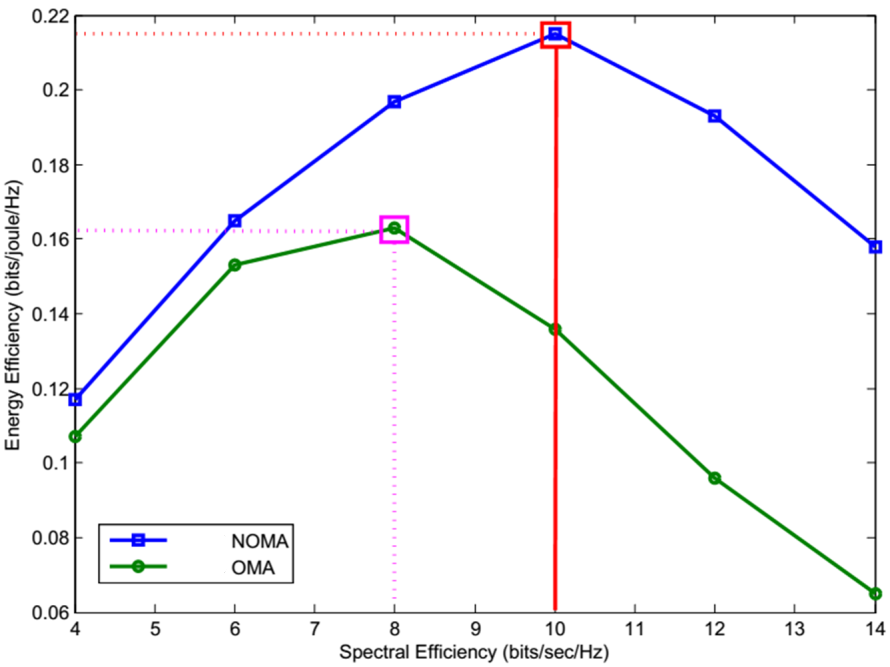
\includegraphics[width=0.7\linewidth]{EEvSE.png}
    \caption[A trade-ff between energy efficiency and spectral effeciency.]{A trade-ff between energy efficiency and spectral effeciency, The peak of the curve (or the corresponding derivative of the EE-SE relationship) is where the system has the maximum energy efficiency \cite{kizilirmak2016noma}.}
    \label{fig:eese}
\end{figure}


NOMA's approach to power management, including dynamic power allocation between users, enables it to achieve any desired point on the EE-SE curve for maximum EE. This is facilitated by varying the total power through power-control schemes, allowing the system to adjust efficiency levels based on specific requirements.

Comparative analyses with OFDMA have demonstrated that NOMA outperforms in terms of EE-SE trade-offs, especially in high Signal to Noise Ratio (SNR) conditions. depicted in \autoref{fig:eese}.
\subsection{Main Advantages of PD-NOMA}

As NOMA continues to evolve in both theoretical and practical aspects, it is increasingly being proposed for next-generation networks. Unlike traditional OMA schemes where the strongest user typically benefits from the highest power, NOMA structures its transmissions differently to provide several distinct advantages summarized as:

\begin{itemize}
    \item \textbf{High Bandwidth Efficiency:} NOMA exhibits high bandwidth efficiency, enhancing the system's overall throughput. This improvement is due to NOMA's ability to allow each Resource Block (RB), such as time or frequency slots, to be shared by multiple users \cite{noma3}.
    \item \textbf{Fairness:} A fundamental aspect of NOMA is its power allocation policy, which tends to favor weaker users, thereby ensuring a more equitable distribution of throughput among all users. This is supported by sophisticated power allocation (PA) policies and the cooperative NOMA schemes that will be further discussed in this paper \cite{noma2}.
    \item \textbf{Ultra-high Connectivity:} With the anticipated rise of the \textit{Internet of Things} (IoT) and the expected connection of billions of smart devices, NOMA offers a promising solution for efficiently managing such extensive connectivity. Unlike conventional OMA, which requires as many frequency/time RBs as there are devices, NOMA can serve a much larger number of devices using fewer RBs by exploiting its non-orthogonal characteristics \cite{liu2020noma}.
    \item \textbf{Compatibility:} From a theoretical standpoint, NOMA can be integrated as an “add-on” technique alongside existing OMA techniques such as TDMA, FDMA, CDMA, and OFDMA. This compatibility is feasible because NOMA operates in a new dimension—the power-domain—complementing the well-established SC and SIC techniques \cite{makki2020survey}.
    \item \textbf{Flexibility:} PD-NOMA is conceptually simpler and generally incurs a lower design complexity compared to other NOMA variants like \textit{Multi-User Shared Access} (MUSA), \textit{Pattern Division Multiple Access} (PDMA), and \textit{Sparse Code Multiple Access} (SCMA). Although these schemes share the fundamental principle of assigning multiple users to a single RB, NOMA's approach, particularly when compared to SCMA, offers straightforward integration of coding, modulation, and subcarrier allocation, making it notably flexible \cite{nagma2}.
\end{itemize}

These advantages position PD-NOMA as a highly effective strategy for enhancing the capabilities of Next-Gen networks, addressing both capacity and performance challenges in densely populated user environments and device-heavy areas such as those anticipated with the expansion of IoT.


\section{Challenges of Multi-User Detection in Uplink}

Multi-user detection in uplink scenarios presents numerous challenges that are critical to the performance and reliability of communication systems, especially in environments with high user density and diverse service requirements. This section explores these challenges, firstly by emphasizing the pivotal role of channel state information (CSI) and modeling. Then we discuss the traditional and optimal detection methods

\subsection{Channel Models and Estimation }

Accurate channel modeling is crucial for studying multi-user detection in uplink scenarios. This modeling involves understanding various channel impairments such as noise, fading, and interference, which affect the quality and reliability of transmitted signals.
\subsubsection*{Rayleigh Fading}

Rayleigh fading is a statistical model used for describing the impact of multipath reception in wireless communications. It assumes that the magnitude of a signal that has undergone multipath propagation will vary randomly according to a Rayleigh distribution. This model is particularly applicable in environments without a direct line of sight between transmitter and receiver.

\begin{equation}
p_R(r) = \frac{2r}{\Omega} e^{-\frac{r^2}{\Omega}} \quad \text{for } r \geq 0
\end{equation}

Where \( \Omega \) is the expected value of \( R^2 \), representing the total power of the signal received through multiple paths. Rayleigh fading is assumed when there is no dominant propagation path, and the small-scale variations in the channel are modeled as Gaussian processes \cite{rayleigh}.
\autoref{fig:log} illustrates the impact of these small-scale variations on the channel gain.
\begin{figure}[H]
    \centering
    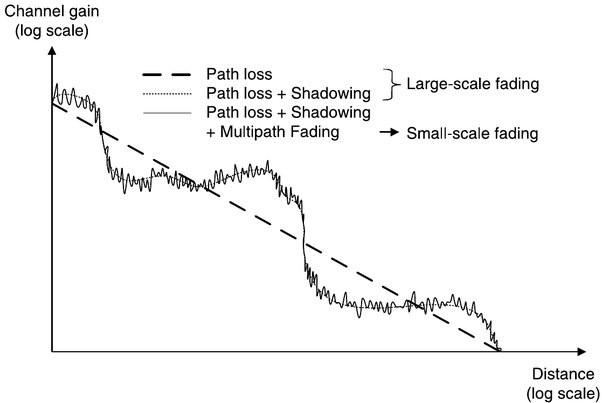
\includegraphics[width=0.75\linewidth]{log.jpg}
    \caption{Channel gain variation with distance.}
    \label{fig:log}
\end{figure}

\subsubsection*{Path Loss and Propagation Models}

Path loss is a critical factor in determining the quality and reliability of the signal received in a mobile communication system. It is essential to use accurate path loss models to predict how the signal degrades over distance, which in turn helps in estimating the Signal-to-Noise Ratio (SNR) for various transmission scenarios.

One of the common path loss models is the Log-distance Path Loss Model. This model is based on empirical measurements and predicts that the average received signal power decreases logarithmically with distance. The path loss can be expressed as:
\begin{equation}
\overline{PL}(dB) = \overline{PL}(d_0) + 10n\log\left(\frac{d}{d_0}\right)
\end{equation}

The bars in this equation denote the ensemble average of all possible path loss values for a given value of \(d\). When plotted on a log-log scale, the modeled path loss is a straight line with a slope equal to \(10n\) dB per decade, this can be observed in \autoref{fig:log} where the dashed line represents the channel gain large-scale variation caused by the path-loss with distance. This modeling approach allows for a simplified yet effective representation of path loss across various environments \cite{rappaport2001wireless}. Here, \( \overline{PL}(dB) \) is the path loss in decibels, \( \overline{PL}(d_0) \) is the path loss at a reference distance \(d_0\), \(n\) is the path loss exponent that characterizes how the path loss increases with distance, and \(d\) is the transmitter-receiver (T-R) separation distance. The value of \(n\) varies based on specific environmental conditions.

Below is a table that lists typical path loss exponents obtained in various mobile radio environments, formatted according to your specified design:

\begin{table}[h]
\centering
\caption{Path loss exponents for different environments \cite{rappaport2001wireless}.}
\label{tab:path_loss_exponents}
\begin{tabular}{@{}lcc@{}}
\toprule
\textbf{Environment} & \textbf{Path Loss Exponent, \(n\)} \\
\midrule
Free space & 2 \\
Urban area cellular radio & 2.7 to 3.5 \\
Shadowed urban cellular radio & 3 to 5 \\
In building line-of-sight & 1.6 to 1.8 \\
Obstructed in building & 4 to 6 \\
Obstructed in factories & 2 to 3 \\
\bottomrule
\end{tabular}
\end{table}
\subsubsection*{Additive White Gaussian Noise (AWGN)}

Additive White Gaussian Noise (AWGN) is a fundamental noise model used in information theory to represent the effect of many random processes that occur in nature. The term "additive" indicates that this noise is added to any intrinsic noise within the information system. "White" suggests that it has uniform power spectral density across the frequency band, similar to white light which contains all visible frequencies. "Gaussian" refers to the normal distribution of the noise's amplitude over time, centered around zero, meaning it is a Gaussian process.

AWGN arises from various natural sources like thermal vibrations of atoms in conductors (thermal noise), shot noise, and radiation from celestial bodies. It is predominantly used as a channel model where the primary impairment to communication is the linear addition of noise with constant spectral density and a Gaussian distribution of amplitude. Although simple, AWGN models are foundational because they provide insight into system behavior under idealized conditions without considering complexities like fading or interference.

\begin{equation}
f_x(x) = \frac{1}{\sqrt{2\pi \sigma_x^2}} \exp\left(-\frac{x^2}{2\sigma_x^2}\right)
\end{equation}

Here, \( \sigma_x^2 \) represents the variance of the noise. The noise in AWGN is characterized as:

\begin{equation}
y_n = x_n + w_n
\end{equation}

Where \( x_n \) is the transmitted signal, typically following a specific modulation scheme, and \( w_n \) represents the AWGN. The effectiveness of the AWGN model is often quantified by the Signal-to-Noise Ratio (SNR), which compares the level of the desired signal to the level of background noise.
\begin{figure}[H]
    \centering
    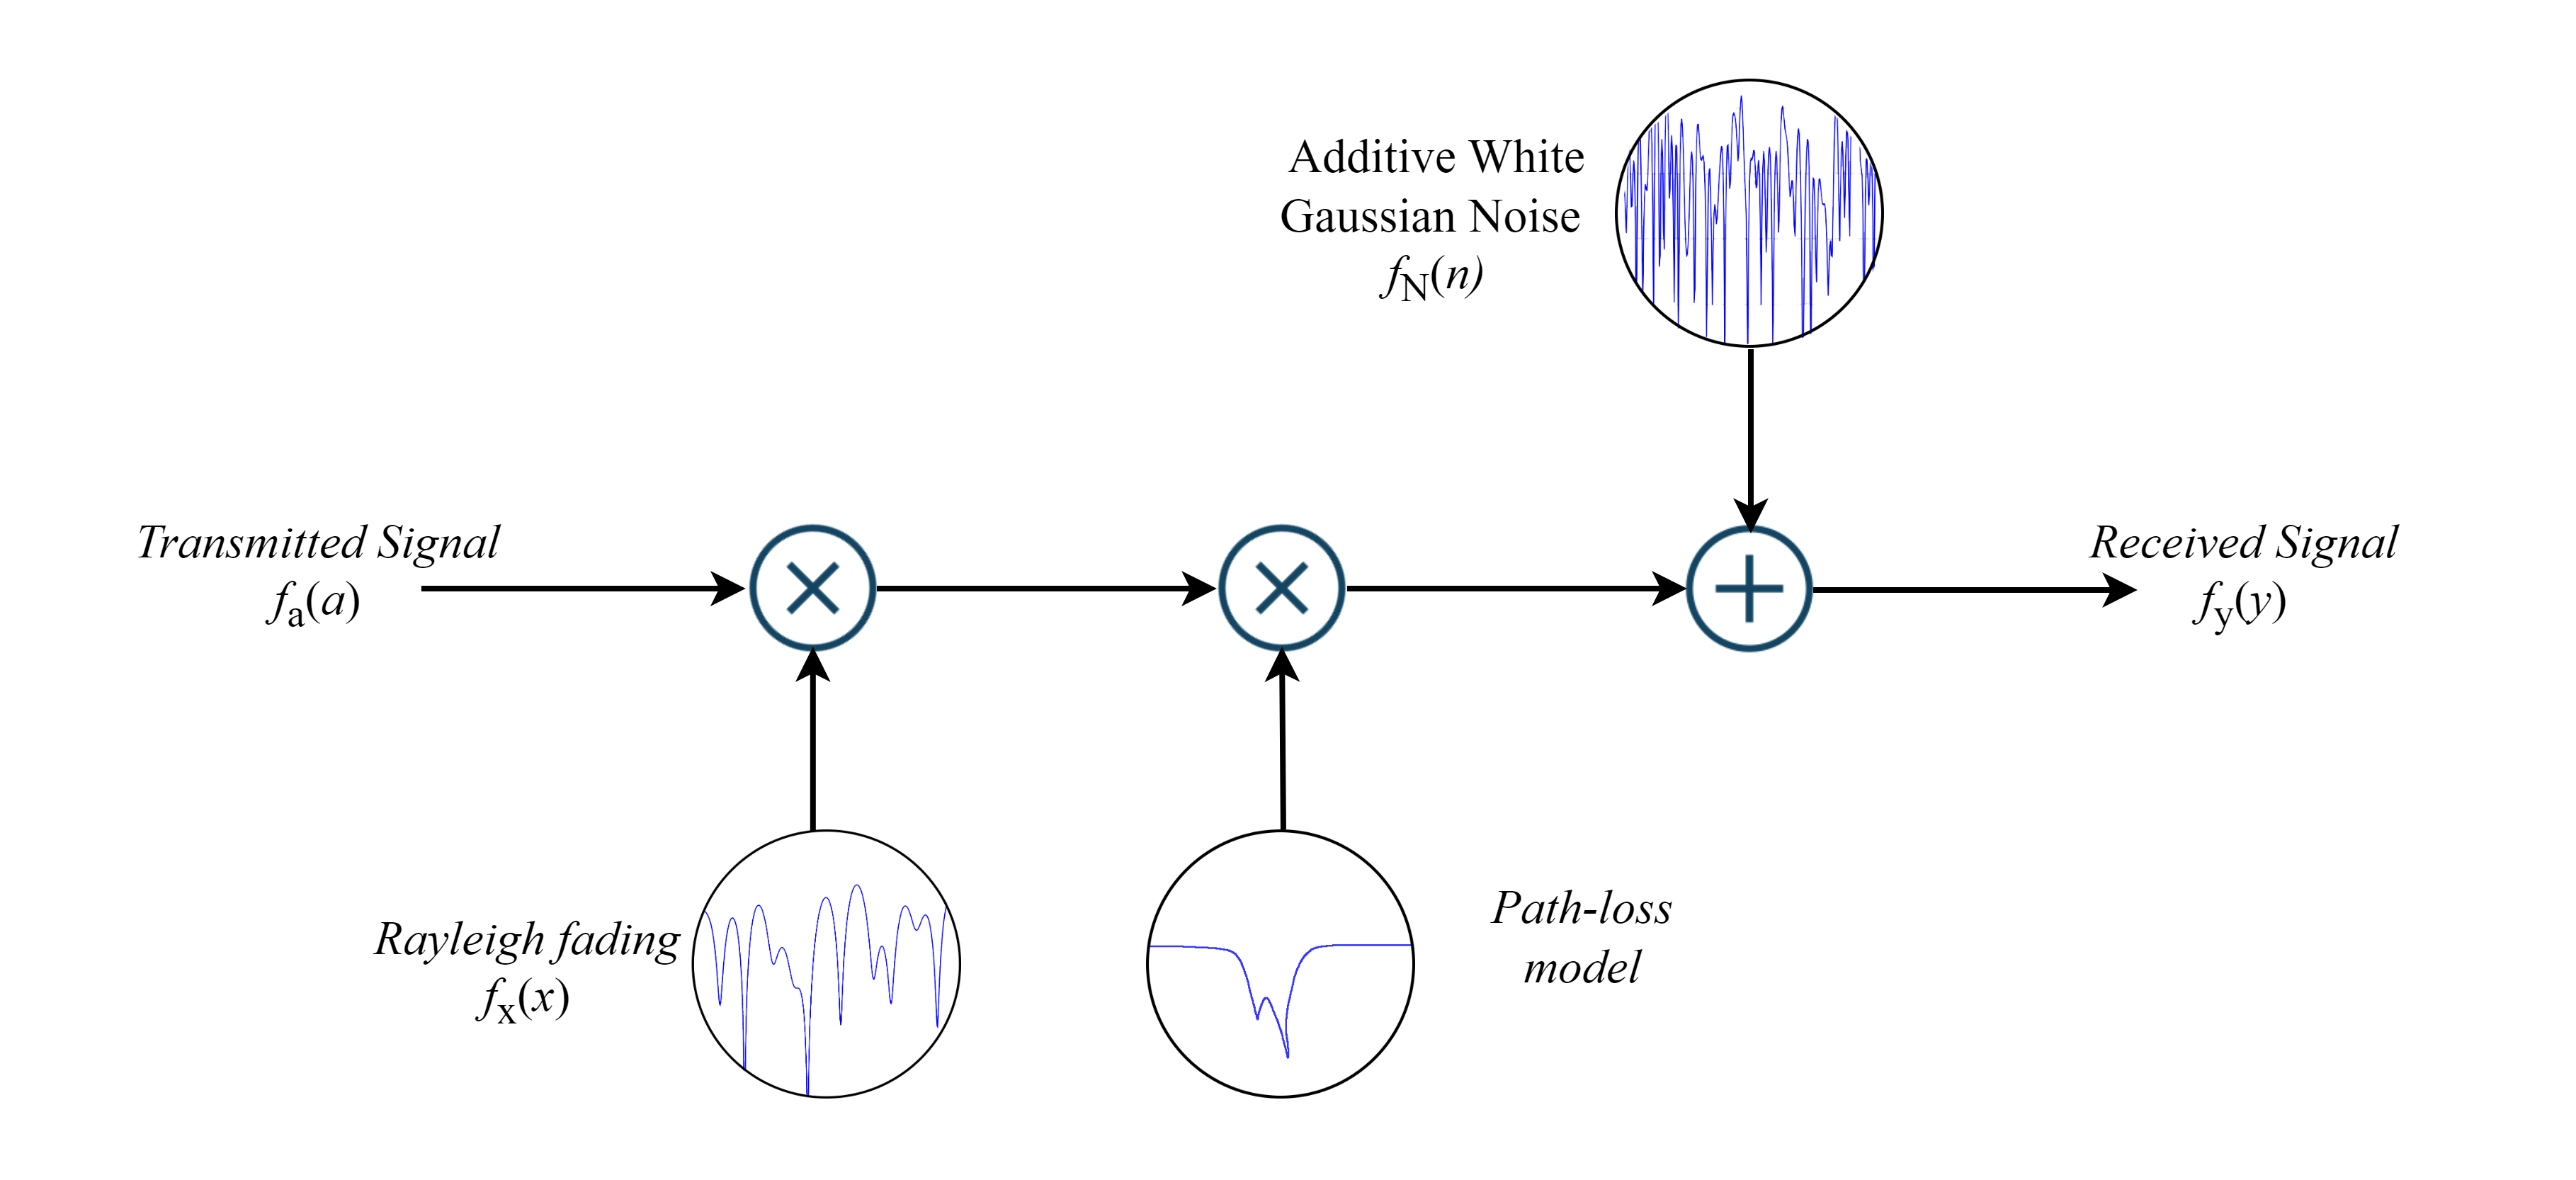
\includegraphics[width=1\linewidth]{Chapter2/Figs/channel model.png}
    \caption{The considered channel model.}
    \label{fig:channel model}
\end{figure}
These models combined -as illustrated in \autoref{fig:channel model}- collectively contribute to our understanding of the uplink channel in multi-user environments.

\subsection*{Importance of Channel Estimation in Uplink Communications}
Channel estimation plays a more significant role in NOMA than in OMA systems, especially for Uplink.  At the base station, precise channel estimation is required to predict and mitigate the effects of the channel as signals arrive. any inaccuracy in estimating the channels between the antennas of all users and the base station can significantly degrade the performance of \textit{Multi-User Detection} (MUD) systems, since the channel estimation errors will result in ambiguous user ordering as well as inaccurate power control, which will in turn affect the SIC decoding accuracy. Naturally, perfect CSI cannot obtained in practice. High
performance near-optimal conventional channel estimation algorithms impose an unacceptable system
overhead and computational complexity on NOMA systems, especially for MIMO-NOMA scenarios. 
\\In our study, particularly in the simulations discussed in Chapter 4, we use the aforementioned channel model for constructing the signal and we assume perfect channel estimation at the BS to focus on evaluating the performance of NOMA MUD under ideal conditions. This assumption allows us to isolate the impact of channel estimation accuracy on system performance and explore potential optimizations in a controlled environment.


\subsection{The Shortcomings of SIC and Conventional Detection Methods}
%Addressing the Performance Downsides of SIC and Conventional Detection Methods
Multi-user detection (MUD) in wireless communication systems is a significant challenge, particularly pronounced in the context of NOMA and Orthogonal OMA systems. In OMA systems like Code Division Multiple Access (CDMA), Orthogonal Frequency Division Multiple Access (OFDMA), Single-Carrier Frequency Division Multiple Access (SC-FDMA), or Time Division Multiple Access (TDMA), users are allocated resources either in a round-robin fashion or allowed to share orthogonal resources simultaneously. For instance, TDMA allocates the entire bandwidth to a single user for specific time slots, while in CDMA, all users simultaneously use the entire bandwidth with unique orthogonal spreading codes.

In contrast, NOMA allows users to share the same frequency and time resources to enhance cell throughput and support more simultaneous users. This necessitates advanced MUD techniques at the base station to accurately extract each user's signal from the  received superposition of signals.\footnote{Please note that the mentioned superposition of signals is their addition
in the classical domain, since in a synchronous system the signals arrive
simultaneously. It should not be confused with the superposition of quantum
states explained in detail in \autoref{chapter: QA}.} Each user transmits its own symbol based on its constellation, and these signals are combined at the receiver, where they are also influenced by Additive White Gaussian Noise (AWGN).
 \begin{figure}[H]
    \centering
    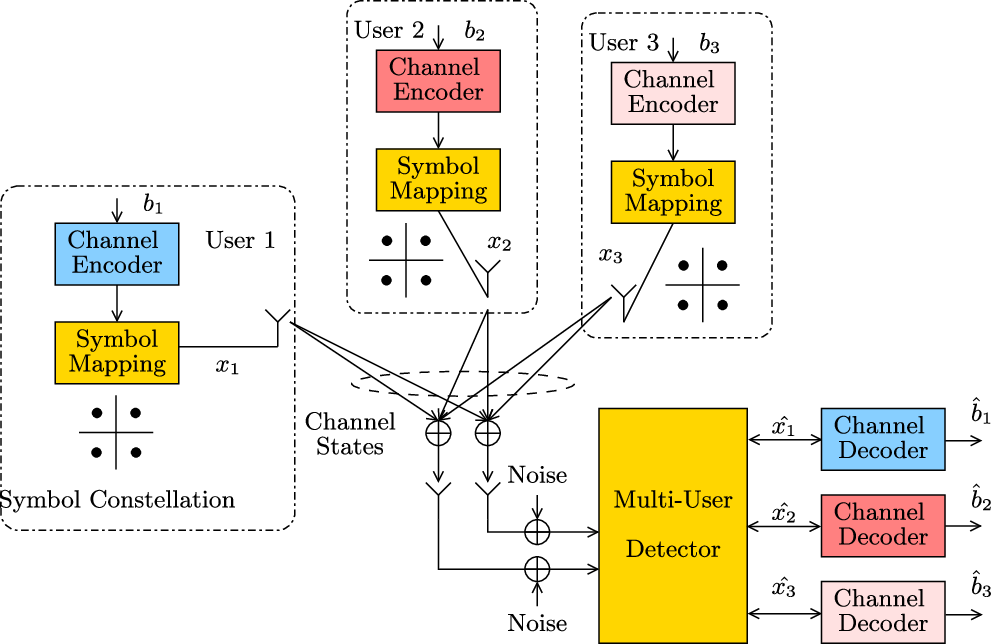
\includegraphics[width=0.75\linewidth]{MUD.png}
    \caption{Uplink system model \cite{QAMUD}.}
    \label{fig:enter-label}
\end{figure}

\textbf{Challenges with Successive Interference Cancellation (SIC):} As previously discussed, SIC has been recognized as a potential decoding solution for NOMA. However, it presents several well-known drawbacks, which become exacerbated as the number of users increases:
\begin{itemize}
    \item The error made in each iteration of SIC can propagate through subsequent iterations, compounding inaccuracies.
    \item Complete channel information must be known at the receiver to perform SIC effectively.
    \item The decoding time increases with the number of users, potentially violating strict latency requirements.
    \item A significant difference in the power levels of each signal is required for successful detection \cite{Kizilirmak2020}.
\end{itemize}

Despite its potential, the implementation of SIC in current wireless systems remains impractical due to high computational costs, latency, and error propagation issues. These challenges have been noted by industry experts and scholars, and even in the latest 5G 3GPP Release 15, NOMA was thoroughly considered but not continued as a work item. The major reasons cited include high implementation complexity required by SIC receivers, significant error propagation in iterative decoding, and high latency were noted as the major reasons for their decision \cite{makki2020survey}.

Efforts to mitigate the load on SIC receivers include user grouping to create parallel channels, which can then be decoded separately using techniques such as beamforming, multicarrier transmission, or Multiple Input Multiple Outputs (MIMO) support \cite{NAGMA}.

Given these significant challenges with SIC, the next logical step is to consider Maximum Likelihood (ML) decoding. ML decoding supports high-quality decoding by effectively managing the complexities associated with multi-user environments without the drawbacks of SIC. This approach is considered next as it offers a robust alternative capable of addressing the stringent demands of modern wireless communication systems.
\subsection{Maximum Likelihood Detection }

The \textit{Maximum Likelihood detection} method represents an optimal approach for MUD in communication systems, particularly effective in distinguishing among the signals transmitted by multiple users in both Orthogonal Multiple Access (OMA) and Non-Orthogonal Multiple Access (NOMA) environments. It is optimal in the sense that it minimizes the
error probability of the detection.

\subsubsection*{Operational Principle of ML Detection}

ML detection seeks to identify the most likely symbol vector transmitted by users, based on the received signal alongside channel estimates. It achieves this by evaluating all conceivable multi-user symbol combinations that could have resulted in the observed reception, thereby selecting the combination that maximizes the likelihood function for a symbol vector \(\mathbf{a}_n\) given the received signal \(\mathbf{y}_n\) \( p(y_n | a_n) \) and the channel gains \(\mathbf{h}_n\) :

\begin{equation}
\hat{\mathbf{a}}_n = \arg\max_{\mathbf{a}_n \in \mathcal{X}^U} \left\{ -\|\mathbf{y}_n - \mathbf{H}_n \mathbf{a}_n\|^2 \right\}
\end{equation}

Here, \(\mathcal{X}\) denotes the constellation set, \(U\) is the number of symbol vectors considered (number of users), \(\mathbf{a}_n\) includes the symbols on the n-th subcarrier, and \(\mathbf{H}_n\) represents the corresponding channel gain matrix. The optimal symbol vector is then forwarded to the channel decoder for subsequent processing \cite{ML1}.

The search space $\mathbb{S}\subseteq\mathcal{X}^U$ contains the candidate vectors. For each $\mathbf{a}_n$, the detector evaluates $\mathcal{D}(\mathbf{a}_n)=\|\mathbf{y}_n-\mathbf{H}_n\mathbf{a}_n\|^2$ and selects the minimum. An exhaustive search uses $\mathbb{S}=\mathcal{X}^U$.



\subsubsection*{Complexity and Performance}

The computational complexity of ML MUD is notably high, for a system supporting \(U\) users, each transmitting symbols from a set \(\mathcal{X}\), scales exponentially with the number of users and symbol choices, making it highly complex. For example, if each of the \(U = 20\) users transmits symbols using 4-ary Quadrature Phase Shift Keying (QPSK), then the ML detector must evaluate \(4^{20}\) (more than one trillion) potential symbol vectors to determine the most likely one. Generally, the complexity can be described as \(O(|\mathcal{X}|^U)\), where \(|\mathcal{X}|\) is the cardinality of the symbol set and \(U\) is the length of the symbol vector.
In contrast, in OMA systems where each received signal typically conveys information from a single user, the complexity of ML MUD is considerably lower, approximately \(O(\mathcal{X}\))), which is manageable given that \(\mathcal{X}\) corresponds to the size of the symbol set used by individual users.
Comparatively, the complexity of Successive Interference Cancellation (SIC) scales linearly with the number of users and symbol length as \(O(|\mathcal{X}| \cdot U)\).
Although SIC has lower computational demands, it performs poorly under conditions where channels have similar characteristics or are rank-deficient, and it is prone to error propagation across decoding stages \cite{ML2}.



ML detection substantially outperforms SIC regarding Bit Error Rate (BER) performance due to its exhaustive approach in evaluating all symbol combinations and its superior handling of channel and noise effects. However, the trade-off involves significantly higher computational demands, particularly challenging in NOMA systems with many users or extensive symbol constellations. Therefore, while ML detection offers enhanced accuracy and superior performance, its practical deployment is often limited by computational capabilities, especially in large-scale user environments, which is the issue we seek to solve in this project \cite{ml}.







